Vidutinio mėnesinio saulės dėmių skaičiaus duomenys\cite{sunspots} 1880 - 2016 metais lyginami su
globalios mėnesinės temperatūros vidutinės anomalijomis\cite{temp} tuo pačiu laikotarpiu.

\begin{figure}
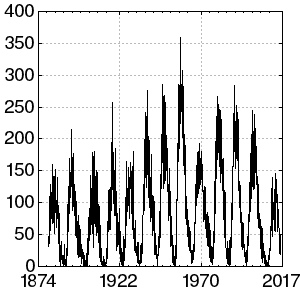
\includegraphics[scale=0.65]{../scripts/sunspots_temperature/sunspots.png}
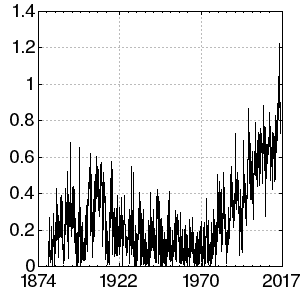
\includegraphics[scale=0.65]{../scripts/sunspots_temperature/temp.png}
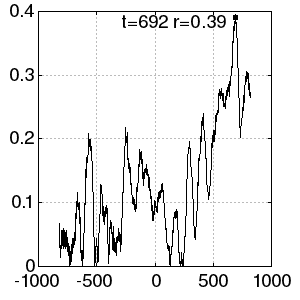
\includegraphics[scale=0.65]{../scripts/sunspots_temperature/result.png}
\caption{Grafikas kairėje: vidutinis mėnesinis saulės dėmių skaičius. Grafikas centre: globalios mėnesinės temperatūros vidutinės anomalijos. Grafikas dešinėje: signalų tarpusavio koreliacija.}
\end{figure}

Signalų poros koreliacijos funkcija rodo didžiausią signalų panašumą \( R_{fg}(t) = 0.39 \), kai \( t = 692 \).
\( R_{fg}(t)\) rodo silpną statistinį ryšį. Bet \(t\) yra apie 57 metai.
Tai per didelis poslinkis.
Saulės aktyvumas kinta periodiškai kas vienuoliką metų.
Poslinkis \(t\) turėtų būti \(< 122 \) mėnesių.
Esant tokiems rezultatams galima konstatuoti, kad koreliacijos tarp saulės aktyvumo ir temperatūros anomalijų nėra arba reikia smulkesnės analizės.
Panašias išvadas pateikia kitas tyrimas\cite{temp_study}.
